\section{Radio Astronomy}\label{ra}
%--------------------------------------------------------------------------------------
\subsection{Radio Telescopes}\label{ra:sec:rt}
%
\subsubsection{Design}\label{ra:ssec:des}
%
\subsubsection{The SKA}
The SKA project was launched in order to create the world's largest array of radio telescopes. This will be achieved by having 197 radio telescopes situated in South Africa and Australia working together and covering an area close to one square kilometre. The array is set to have a resolution of over 50 times that of the Hubble Space Telescope while still covering massive areas of the sky (\cite{SKAsite}).
%--------------------------------------------------------------------------------------
\subsection{Image Capturing}\label{ra:sec:ic}
%
\subsubsection{The Primary Beam}\label{ra:ssec:tpb}
The primary beam is a mathematical function that describes the sensitivity pattern of an antenna. Naturally the beam is most sensitive in the centre of the direction in which it is facing, with fringes of sensitivity radiating out as can be seen in Figure \ref{ra:fig:beam}. The circular sensitivity present in Figure \ref{ra:fig:beam} is also due to the fact that the telescope rotates in order to keep the centre of the beam focused on the same area of the sky. The errors produced by the lack of sensitivity in certain areas can be compensated for, but that lies outside the scope of this paper (\citet{oleg}).
%
\begin{figure}[H]
	\centering
	\label{ra:fig:beam}
	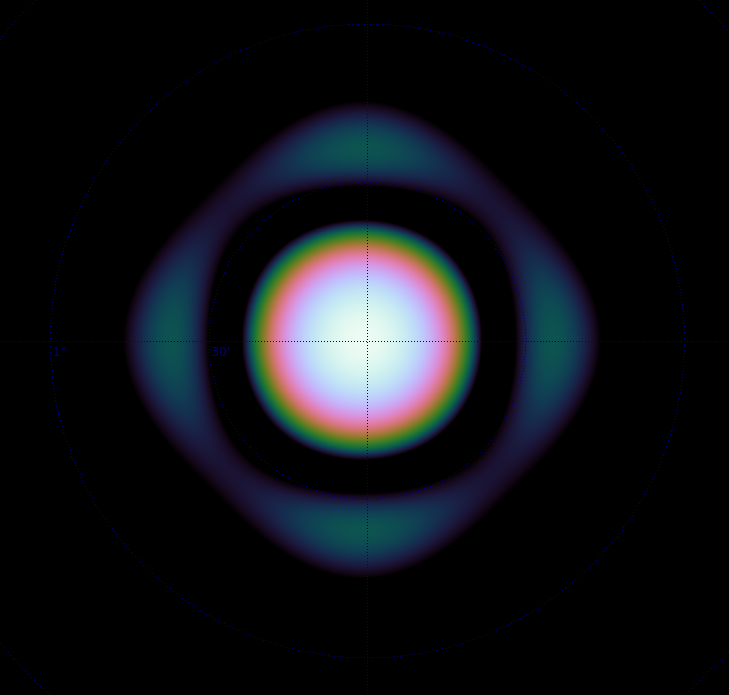
\includegraphics[scale=0.28]{Images/beam.png}
	\caption{Primary Beam Focus Pattern(\cite{oleg})}
\end{figure}
%--------------------------------------------------------------------------------------
\subsection{Image Processing}\label{ra:sec:img}
%
\subsubsection{Methods}\label{ra:ssec:meth}
%
\subsubsection{Errors}\label{ra:ssec:err}
%
\subsubsection{Error Correction}\label{ra:ssec:ec}
%--------------------------------------------------------------------------------------